\section{Rule Chains}
In this project, two distinct nodes were developed, each with its specific characteristics. On one hand, we have a node equipped with sensors for presence detection, 
periodic measurements of temperature, humidity, wind, smoke, and flame detection via infrared sensors, located at the perimeter of the field. On the other hand, a 
simpler node equipped with an accelerometer is placed on the fence delimiting the crop field to detect potential unauthorized crossings. For each of these nodes,
two Device Profiles were defined in Thingsboard: "PIR Node Profile" and "Fence Node Profile". Each profile is assigned a specific Rule Chain to analyze the data 
received from the devices and trigger the corresponding alarms.


\subsection{PIR Node Analyzer}
The alarms generated by this Rule Chain include:
\begin{itemize}
    \item Fire Detected.
    \item Fire Hazard.
    \item Presence Detected.
\end{itemize}

The Rule Chain first validates that all required fields are present in the incoming message. If the message format is incorrect or incomplete, an alarm is triggered 
to indicate that the incoming message cannot be processed. Once the message format is validated, the data is parsed for easier subsequent processing, producing a JSON
structure similar to the one shown in \autoref{fig:parsedJson}.

\begin{figure}[H]
    \centering
    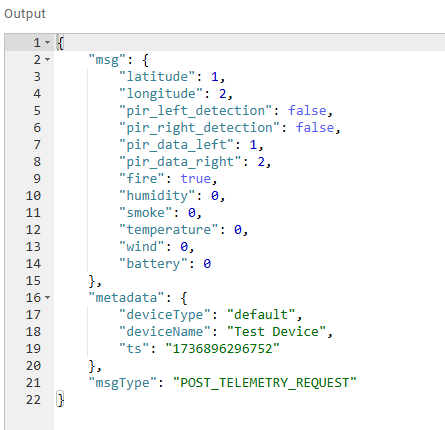
\includegraphics[width=0.3\textwidth]{./images/8/jsonParsed.PNG}
    \caption{Parsed JSON for Rule Chain Processing}
    \label{fig:parsedJson}
\end{figure}

Fire detection relies on the value in the 'fire' field. In the Check Fire node of the Rule Chain, if the 'fire' field returns 'true', a critical alarm for "Fire Detected"
is triggered. If the value is 'false', the alarm is deactivated.

The "Fire Hazard" alarm is activated by evaluating the parameters for temperature, humidity, wind speed, and smoke levels. According to AÑADIR REFERENCIA, the conditions 
for a fire hazard include:
\begin{itemize}
    \item Temperature above 30°C.
    \item Relative humidity below 30\%.
    \item Wind speeds exceeding 30 km/h.
\end{itemize}

Additionally, a smoke concentration exceeding 200 ppm triggers the alarm. If none of these conditions are met, the alarm is deactivated.

For presence detection, four PIR nodes are placed at each vertex of the square representing the crop field. The field is divided into four zones corresponding to each side 
of the polygon. The presence detection algorithm works as follows:
\begin{itemize}
    \item If a presence is detected by a PIR sensor (indicated by 'pir_XX_detection', where XX can be 'left' or 'right'):
    \begin{itemize}
        \item The status of the opposite side’s neighboring node is checked.
        \item If the neighboring node also reports presence ('true') within a timespan of 10 seconds, the "Presence Detected" alarm is triggered, and a speaker is activated.
        \item If no presence is detected on the opposite side, a lower-priority alarm is triggered, indicating presence on one side of the fence.
    \end{itemize}
    \item If no presence is detected on the initial node, all related presence alarms are deactivated. 
\end{itemize}

The pseudocode for this logic is as follows:
\todo[inline]{METER CÓDIGO FORMATEADO}
if (presence on one side):
    if (presence on opposite-side neighbor node && ts < 10):
        Presence Detected
        Activate Speaker
    else:
        Presence Detected on the corresponding side
else:
    Deactivate all presence alarms

To implement this algorithm, relationships between the various nodes and assets were defined. Accessing values from neighboring nodes was achieved through the Change
Originator node in Thingsboard, which specifies the target node using the predefined relationships. Similarly, the originator change process is used to update related 
asset values. The full flow of the Rule Chain is illustrated in \autoref{fig:PirNodeAnalyzer}.

\begin{figure}[H]
    \centering
    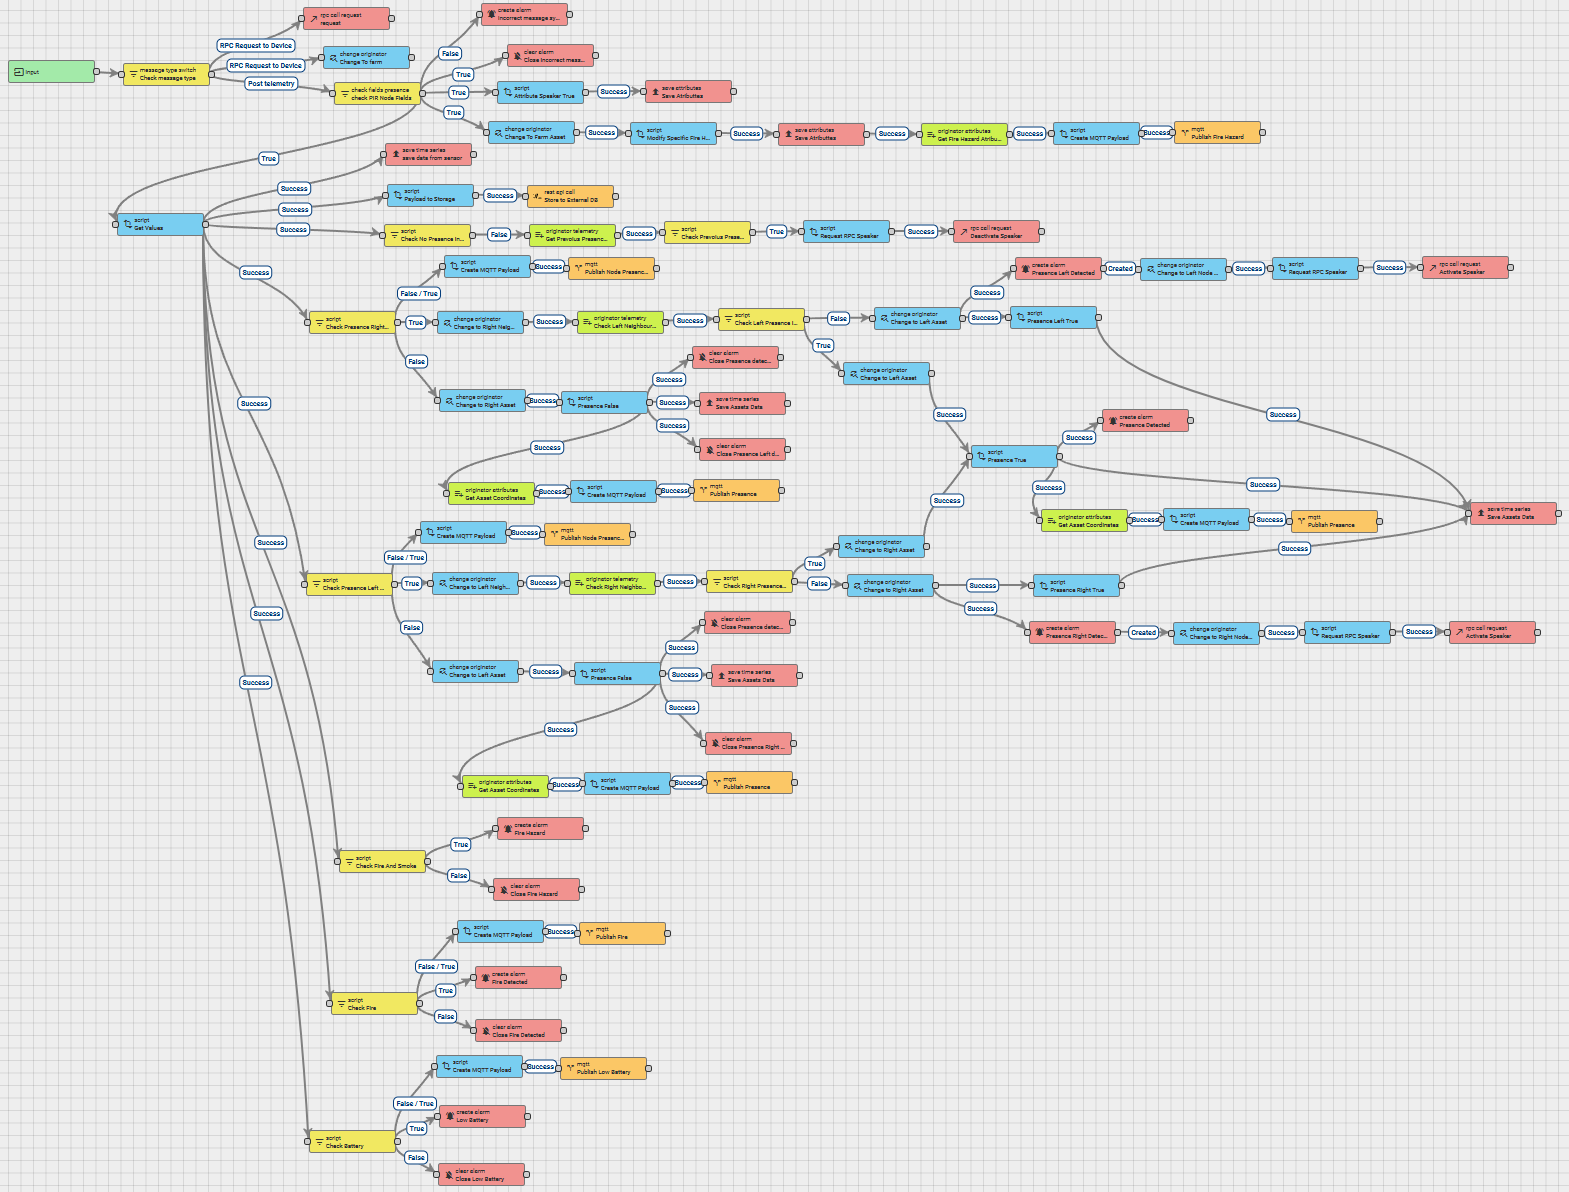
\includegraphics[width=0.3\textwidth]{./images/8/PirNodeAnalyzer.PNG}
    \caption{PIR Node Analyzer Rule Chain FLow}
    \label{fig:PirNodeAnalyzer}
\end{figure}

\subsection{Fence Node Analyzer}
This Rule Chain is designed to process messages from nodes placed on the fence to detect movements and generate alarms accordingly.  
Similar to the previous Rule Chain, it first validates that all required fields are present in the incoming message. However, since this node is simpler, the Rule 
Chain specifically generates the "Fence Trespassed" alarm based on the value of the 'acceleration_interruption' field. The flow of this process is illustrated in \autoref{fig:FenceNodeAnalyzer}.

\begin{figure}[H]
    \centering
    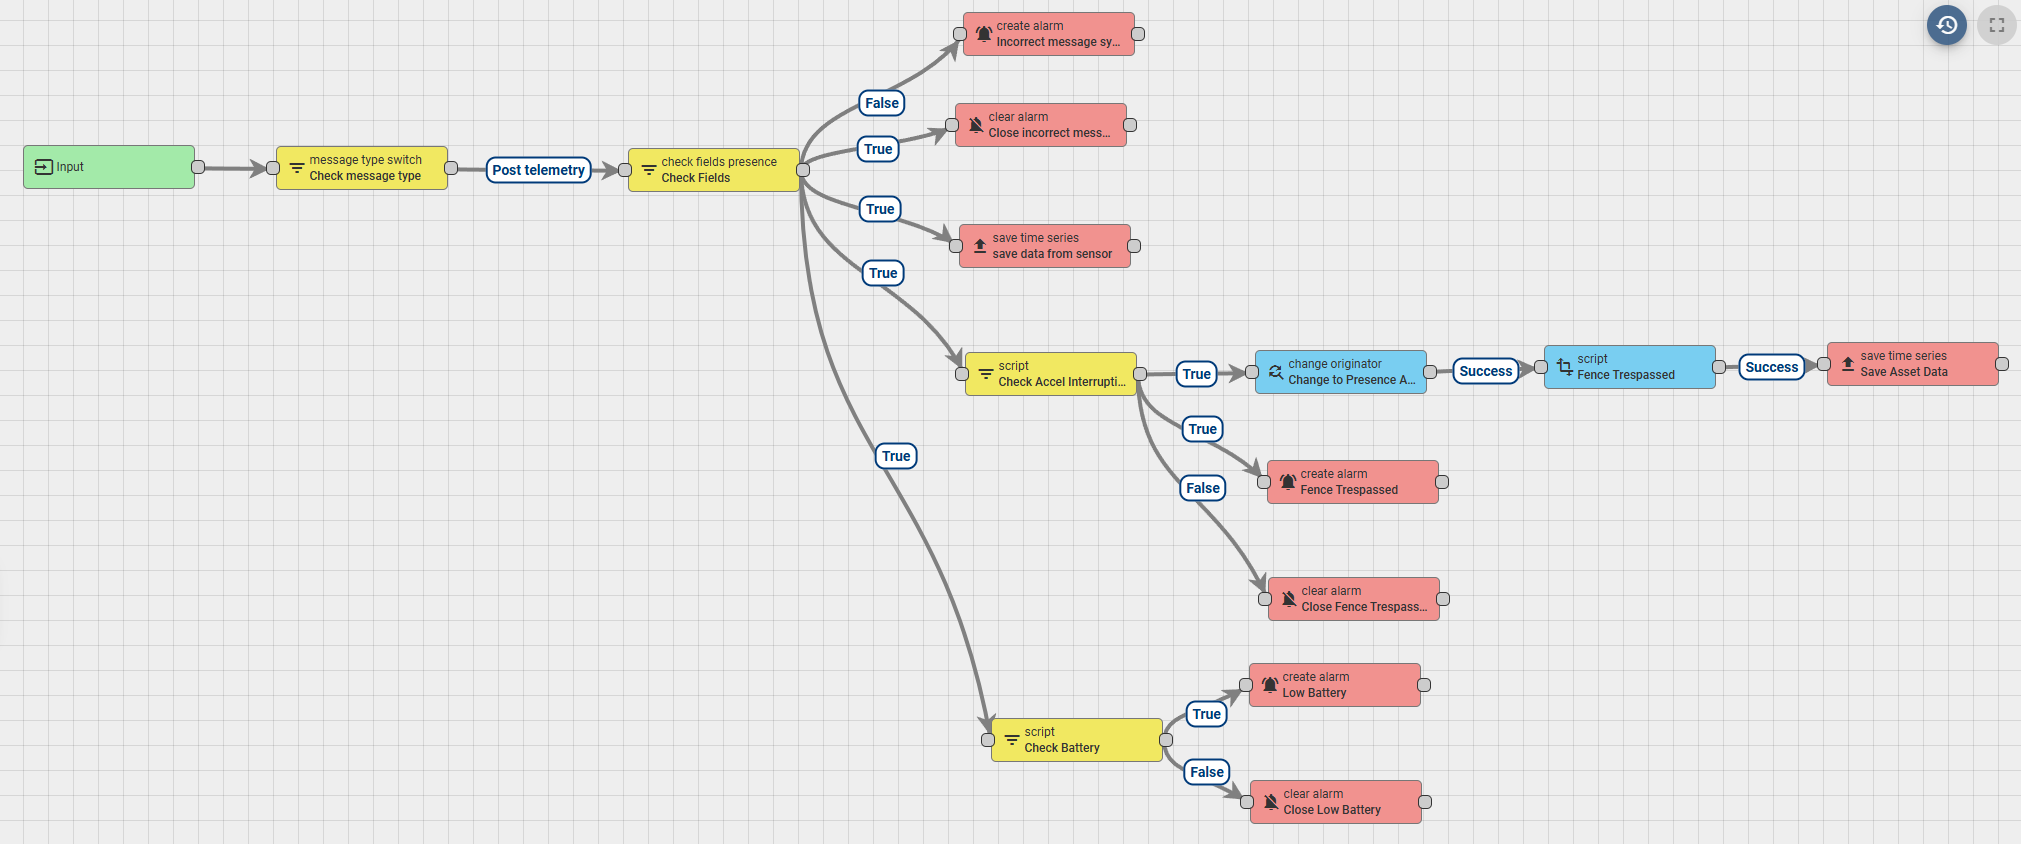
\includegraphics[width=0.3\textwidth]{./images/8/FenceNodeAnalyzer.PNG}
    \caption{Fence Node Analyzer Rule Chain FLow}
    \label{fig:FenceNodeAnalyzer}
\end{figure}